% !TEX root = ../Ausarbeitung.tex
\section{Learned Approaches}
\label{sec:learned}
The next approach tries to learn some of the movements instead of hard-coding them.
An evolutionary approach is used to learn weights for a spiking neural network which controls the robots movements.

\subsection{Evolutionary Approach}
In this approach the robot is controlled by a spiking neural network.
The networks topology is illustrated in \autoref{fig:network}.
It has three input and seven output neurons which are fully connected.
The three dimensional position of the cylinder is used for the input neurons.
Six of the output neurons control the six joints of the robot arm and the last neuron tells the hand when it should release the cylinder.

The absolute value of the cylinders position is directly set as the amplitude of the input neurons.
This results in the spike rate of the neurons increasing as the absolute position values of the cylinder increase.
The spike rate of the first six output neurons is passed to the arm joints as a position which produces a movement of the arm.
The spikes of the seventh output neuron control the release of the cylinder, optimally resulting in the cylinder flying away.

For the evolutionary algorithm, each individual is a list of 21 values, each representing one weight of the network.
To evaluate the individuals, a throw is simulated and the distance of the cylinder from the table is measured, which represents the fitness of the individual.
After each individual of a generation is evaluated, the elite, which consists of the best 50\% of the individuals, is selected.
The elite gets copied into the next generation and the remaining individuals are generated by mutating and recombining the individuals of the elite.

\begin{figure}[h]
\centering
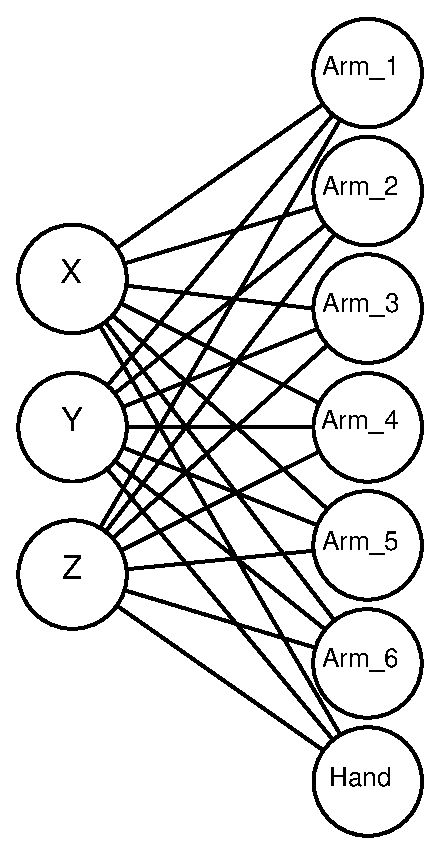
\includegraphics[width=.5\columnwidth]{figures/net.eps}
\caption{The spiking neural network takes the cylinder coordinates $X, Y, Z$ as inputs and has seven outputs controlling the robot arm configuration and the release point.}
\label{fig:network}
\end{figure}

\subsubsection{Mutation Strategies}
Three different mutation strategies are implemented to generate new descendants.
The first method uses only one parent and adds or subtracts small random values from its weights to produce an offspring.
The other two methods are a single-point crossover and a k-point crossover as described in \autoref{sec:ea}.

\subsection{Simplified Problem}
As the first learning approach isn't very successful and it is learning very slowly, a reduction of the number of parameters and thus the search space for the evolutionary algorithm may be beneficial.
To achieve this, some joints are excluded from the throwing motion.
All rotational joints are fixed by setting the respective weights in the neural network to zero, because these probably won't impact the robots ability to make a good throw very much.
This reduces the number of weights to be learned from 21 to 12.